% Template for Cogsci submission with R Markdown

% Stuff changed from original Markdown PLOS Template
\documentclass[10pt, letterpaper]{article}

\usepackage{cogsci}
\usepackage{pslatex}
\usepackage{float}
\usepackage{caption}

% amsmath package, useful for mathematical formulas
\usepackage{amsmath}

% amssymb package, useful for mathematical symbols
\usepackage{amssymb}

% hyperref package, useful for hyperlinks
\usepackage{hyperref}

% graphicx package, useful for including eps and pdf graphics
% include graphics with the command \includegraphics
\usepackage{graphicx}

% Sweave(-like)
\usepackage{fancyvrb}
\DefineVerbatimEnvironment{Sinput}{Verbatim}{fontshape=sl}
\DefineVerbatimEnvironment{Soutput}{Verbatim}{}
\DefineVerbatimEnvironment{Scode}{Verbatim}{fontshape=sl}
\newenvironment{Schunk}{}{}
\DefineVerbatimEnvironment{Code}{Verbatim}{}
\DefineVerbatimEnvironment{CodeInput}{Verbatim}{fontshape=sl}
\DefineVerbatimEnvironment{CodeOutput}{Verbatim}{}
\newenvironment{CodeChunk}{}{}

% cite package, to clean up citations in the main text. Do not remove.
\usepackage{apacite}

% KM added 1/4/18 to allow control of blind submission


\usepackage{color}

% Use doublespacing - comment out for single spacing
%\usepackage{setspace}
%\doublespacing


% % Text layout
% \topmargin 0.0cm
% \oddsidemargin 0.5cm
% \evensidemargin 0.5cm
% \textwidth 16cm
% \textheight 21cm

\title{Quantifying social information in natural infant visual experience}


\author{{\large \bf Bria Long (bria@stanford.edu)}  \AND {\large \bf George Kachergis (kachergis@stanford.edu)}  \AND {\large \bf Ketan Jay Agarwal (agrawalk@stanford.edu)}  \AND {\large \bf Michael C. Frank (mcfrank@stanford.edu)} \\  Department of Psychology, Street Address \\ Stanford, CA 91305 USA}

\begin{document}

\maketitle

\begin{abstract}
The faces and hands of infants' caregivers and other social partners
offer a rich source of social and causal information that may be
critical for infants' cognitive and linguistic development.

\textbf{Keywords:}
social cognition; face perception; infancy; head cameras; deep learning
\end{abstract}

\hypertarget{introduction}{%
\section{Introduction}\label{introduction}}

Infants are famously confronted by a blooming, buzzing onslaught of
stimuli (James, 1891) which they must learn to parse and navigate as
their cognitive and social skills develop. Fortunately, they can depend
on regularities not only in their visual environments (Aslin, 2009) and
linguistic environments, but also in the presence and actions of their
caregivers and other social partners {[}@{]}. From a very young age,
infants show great attention to faces CITE, and indeed faces are a
critical part of infants' visual experience as an important conduit of
social and linguistic information. As infants mature, they begin to also
attend more to the manual actions taken by their social partners,
engaging in joint attention to objects and events around them. Such
episodes are prompted not only by a glance from a caregiver, but also
through pointing and offering; thus, hands are also an important carrier
of information, especially relevant for learning language and actions.
It is unsurprising, then, that both hands and faces are prevalent in
even young infants' visual experiences, as evidenced through analyses of
egocentric views collected with head-mounted cameras (i.e., headcams;
CITES).

Of course, not only is children's interest and attention to hands and
faces

Previous work has suggested:

Previous work has found changes in the prevalence of faces vs.~hands for
infants of different ages. For example, Fausey et al. (2016) found that
infants less than 12 months of age received face-dense input, relative
to 1- to 2-year-olds who received more hand-dense input. However, it may
be that this effect is driven by infants younger than 4 months of age
(e.g., Jayaraman, Fausey, \& Smith, 2015; Sugden, Mohamed-Ali, \&
Moulson, n.d.) who see both more frequent and more persistent faces
(Jayaraman \& Smith, 2018). Once infants begin to crawl
(\textasciitilde{}6 months) they may see far fewer hands and faces,
overall.

Earlier work has also found surprising attention to hand movements and
their interactions with objects (Yu \& Smith, 2013), particularly in
older infants (ages?).

Differences in the availability of social information depending on motor
abilities (Franchak, Kretch, Soska, \& Adolph, 2011; Sanchez, Long,
Kraus, \& Frank, 2018) (more Franchak papers?)

One limitation of past work is that it has relied on cross-sectional
data, and thus cannot speak to whether these trajectories are present in
individual children.

Here, we analyze the SAYcam dataset (Sullivan, Mei, Perfors, Wojcik, \&
Frank, n.d.), a longitudinal corpus of head-mounted camera data
comprising more than 1700 videos from three children, for a total of
over 300 hours of videos (\textgreater{}100 million frames). Over a span
of 6 to 32 months of age, the three children (S, A, and Y) in the
dataset wore headcams at least twice weekly, for approximately one hour
per recording session. One weekly session was on the same day each week
at a roughly constant time of day, while the other(s) were chosen
arbitrarily at the participating family's discretion.

This dataset differs in four key ways: 1) number of hours/frames 2) not
just mealtimes--naturalistic sample of many contexts, 3) longitudinal,
4) much larger field-of-view.

To do so, we first test and validate novel computer vision methods for
extracting social information from these egocentric viewpoints on a
small subset of randomly selected frames from the dataset.\\
We then apply these methods at scale to the larger dataset, allowing us
to extract key descriptive variables hypothesized to vary across
development.

\hypertarget{method}{%
\section{Method}\label{method}}

\hypertarget{dataset}{%
\subsection{Dataset}\label{dataset}}

(briefly describe dataset; sampling strategy: location of two
households, number of hours of video, variability in location, etc;
reference published paper on what this dataset is, large field of view
(fisheye lens)) (109 degrees horizontal x 70 degrees vertical)

\hypertarget{part-1-how-well-can-we-capture-social-information-using-computer-vision}{%
\subsection{Part 1: How well can we capture social information using
computer
vision?}\label{part-1-how-well-can-we-capture-social-information-using-computer-vision}}

\hypertarget{description-of-openpose-figure-1}{%
\subsubsection{Description of OpenPose (Figure
1)}\label{description-of-openpose-figure-1}}

To automatically annotate the millions of frames in SAYcam, we use
OpenPose (Cao, Hidalgo, Simon, Wei, \& Sheikh, 2018; Simon, Joo,
Matthews, \& Sheikh, 2017), a computer vision model optimized for
jointly detecting human face, body, hand, and foot keypoints (135 in
total) that operates well on scenes including multiple people even if
they are partially-occluded.

\hypertarget{description-of-annotation-strategy-24k-by-ketan-4k-on-amazon-mechanical-turk-reliability}{%
\subsubsection{Description of annotation strategy (24K by Ketan, 4K on
Amazon Mechanical Turk,
reliability)}\label{description-of-annotation-strategy-24k-by-ketan-4k-on-amazon-mechanical-turk-reliability}}

To test the validity of OpenPose's hand and face detections, we compared
to human annotations of 24,000 frames selected uniformly at random from
the videos of two children (S and A).

\hypertarget{describe-main-prf-statistics-for-24k-for-faces-and-hands-interpret.}{%
\subsubsection{Describe main PRF statistics for 24K for faces and hands;
interpret.}\label{describe-main-prf-statistics-for-24k-for-faces-and-hands-interpret.}}

Relatively higher precision vs.~recall. - P/R/F variation across
child/age for faces - Describe possible sources of variation that
decrease scores for: - Faces: weird viewpoints, occluded/side viewpoint,
faces in books - Hands: children's own hands, hands in books, side
viewpoints - Describe additional child vs.~hand annotation; P/R/F
variation across child vs.~adult hands (better for adult hands, still OK
for child hands)

\hypertarget{part-2-access-to-social-information-across-age}{%
\subsection{Part 2: Access to social information across
age}\label{part-2-access-to-social-information-across-age}}

\hypertarget{prevalence-of-hands-vs-faces-across-age-in-goldset-full-dataset-figure-2}{%
\subsubsection{Prevalence of hands vs faces across age (in goldset, full
dataset) (Figure
2)}\label{prevalence-of-hands-vs-faces-across-age-in-goldset-full-dataset-figure-2}}

\hypertarget{why-so-many-hands}{%
\subsubsection{Why so many hands?}\label{why-so-many-hands}}

\hypertarget{more-child-hands-as-in-gold-set}{%
\subsubsection{More child hands as in gold
set}\label{more-child-hands-as-in-gold-set}}

\hypertarget{field-of-view-comparison}{%
\subsection{Field-of-View Comparison}\label{field-of-view-comparison}}

The field of view (FOV) of the fisheye lens used in Sullivan et al.
(n.d.) is much wider (109 degrees horizontal x 70 degrees vertical) than
the FOV of the lens used in Fausey et al. (2016) (69 deg. x 41 deg.).
Looks like child hands make up about \textasciitilde{}34\% of the hands
detected in our gold set (in Fausey 2016, they are only 8\% of the
hands). Furthermore, a lot of the lower proportions of hands come from
the infants \textless{}6 months of age.

\hypertarget{variability-by-location}{%
\subsection{Variability by Location}\label{variability-by-location}}

Next we examine variation in the presence of hands and faces across
different locations. Of the 3,027 videos, the content of 1,829 have been
manually manuallly annotated for filming location, activities taking
place, and visible objects (see Sullivan et al. (n.d.)). To give a sense
of the contexts the children experienced, the most frequent filming
locations were the living room (339 videos), bedroom (182), kitchen
(150), outside on property (129), child's bedroom (81), deck/porch (73),
hallway (70), and off property (57). Filming only took place twice in
the dining room.

The most frequent activities were sitting (410), playing (375), being
held (352), and standing (297). Eating was the 11th most-frequent
activity (117 videos).

(goldset, full dataset)

List multiple references alphabetically and separate them by semicolons
(Frank, 2012; Smith, Yu, \& Pereira, 2011).

You might want to display a wide figure across both columns. To do this,
you change the \texttt{fig.env} chunk option to \texttt{figure*}. To
align the image in the center of the page, set \texttt{fig.align} option
to \texttt{center}. To format the width of your caption text, you set
the \texttt{num.cols.cap} option to \texttt{2}.

\hypertarget{one-column-images}{%
\subsection{One-column images}\label{one-column-images}}

Single column is the default option, but if you want set it explicitly,
set \texttt{fig.env} to \texttt{figure}. Notice that the
\texttt{num.cols} option for the caption width is set to \texttt{1}.

\begin{CodeChunk}
\begin{figure}[H]

{\centering 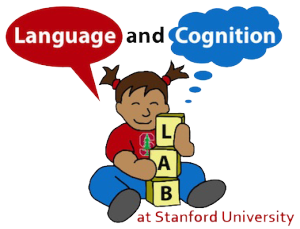
\includegraphics{figs/image-1} 

}

\caption[One column image]{One column image.}\label{fig:image}
\end{figure}
\end{CodeChunk}

\hypertarget{r-plots}{%
\subsection{R Plots}\label{r-plots}}

You can use R chunks directly to plot graphs. And you can use latex
floats in the fig.pos chunk option to have more control over the
location of your plot on the page. For more information on latex
placement specifiers see
\textbf{\href{https://en.wikibooks.org/wiki/LaTeX/Floats,_Figures_and_Captions}{here}}

\begin{CodeChunk}
\begin{figure}[H]

{\centering 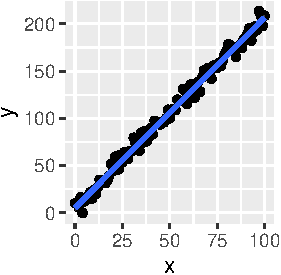
\includegraphics{figs/plot-1} 

}

\caption[R plot]{R plot}\label{fig:plot}
\end{figure}
\end{CodeChunk}

\hypertarget{tables}{%
\subsection{Tables}\label{tables}}

You can use the xtable function in the xtable package.

\begin{table}[H]
\centering
\begin{tabular}{rrrrr}
  \hline
 & Estimate & Std. Error & t value & Pr($>$$|$t$|$) \\ 
  \hline
(Intercept) & -0.09 & 0.10 & -0.9 & 0.35 \\ 
  x & 2.06 & 0.11 & 18.5 & 0.00 \\ 
   \hline
\end{tabular}
\caption{This table prints across one column.} 
\end{table}

\hypertarget{discussion}{%
\section{Discussion}\label{discussion}}

Fausey 2016: 103,383 images; Here: 30,000,000 frames; 300 fold increase
in data

\hypertarget{acknowledgements}{%
\section{Acknowledgements}\label{acknowledgements}}

We would like to thank X and Y for helpful comments, and\ldots{}

\hypertarget{references}{%
\section{References}\label{references}}

\setlength{\parindent}{-0.1in} 
\setlength{\leftskip}{0.125in}

\noindent

\hypertarget{refs}{}
\leavevmode\hypertarget{ref-Aslin2009}{}%
Aslin, R. N. (2009). How infants view natural scenes gathered from a
head-mounted camera. \emph{Optometry and Vision Science: Official
Publication of the American Academy of Optometry}, \emph{86}(6),
561--565.

\leavevmode\hypertarget{ref-Cao2018openpose}{}%
Cao, Z., Hidalgo, G., Simon, T., Wei, S.-E., \& Sheikh, Y. (2018).
OpenPose: Realtime multi-person 2D pose estimation using Part Affinity
Fields. In \emph{ArXiv preprint arXiv:1812.08008}.

\leavevmode\hypertarget{ref-Fausey2016}{}%
Fausey, C. M., Jayaraman, S., \& Smith, L. B. (2016). From faces to
hands: Changing visual input in the first two years. \emph{Cognition},
\emph{152}, 101--107.

\leavevmode\hypertarget{ref-Franchak2011}{}%
Franchak, J. M., Kretch, K. S., Soska, K. C., \& Adolph, K. E. (2011).
Head-mounted eye- tracking: A new method to describe infant looking.
\emph{Child Development}, \emph{82}(6), 1738--1750.

\leavevmode\hypertarget{ref-Frank2012}{}%
Frank, M. C. (2012). Measuring children's visual access to social
information using face detection. In \emph{Proceedings of the nth annual
conference of the cognitive science society} (pp. XXX--XXX). Hillsdale,
NJ: Cognitive Science Society.

\leavevmode\hypertarget{ref-Jayaraman2015}{}%
Jayaraman, S., Fausey, C. M., \& Smith, L. B. (2015). The faces in
infant-perspective scenes change over the first year of life. \emph{PLoS
One}. \url{http://doi.org/10.1371/journal.pone.0123780}

\leavevmode\hypertarget{ref-Jayaraman2018}{}%
Jayaraman, S., \& Smith, L. B. (2018). Faces in early visual
environments are persistent not just frequent. \emph{Vision Research}.

\leavevmode\hypertarget{ref-Sanchez2018}{}%
Sanchez, A., Long, B., Kraus, A. M., \& Frank, M. C. (2018). Postural
developments modulate children's visual access to social information. In
\emph{Proceedings of the 40th annual conference of the cognitive science
society}.

\leavevmode\hypertarget{ref-Simon2017hand}{}%
Simon, T., Joo, H., Matthews, I., \& Sheikh, Y. (2017). Hand keypoint
detection in single images using multiview bootstrapping. In
\emph{CVPR}.

\leavevmode\hypertarget{ref-Smith2011}{}%
Smith, L. B., Yu, C., \& Pereira, A. (2011). Not your mother's view: The
dynamics of toddler visual experience. \emph{Developmental Science},
\emph{14}(1), 9--17.

\leavevmode\hypertarget{ref-Sugden2014}{}%
Sugden, N. A., Mohamed-Ali, M. I., \& Moulson, M. C. (n.d.). I spy with
my little eye: Typical, daily exposure to faces documented from a
first-person infant perspective. \emph{Developmental Psychobiology},
\emph{56}(2), 249--261.

\leavevmode\hypertarget{ref-SAYcam}{}%
Sullivan, J., Mei, M., Perfors, A., Wojcik, E., \& Frank, M. (n.d.).
Head cameras on children aged 6 months through 31 months.

\bibliographystyle{apacite}


\end{document}
